\section{Screening Applications}
\label{sec:screening}

\subsection{Imidazolium ILs}
The Random Forest trained on all data was used to rank 25 combinations of five 1-alkyl-3-methylimidazolium cations ([EMIM], [PMIM], [BMIM], [HMIM], [OMIM]) and five anions ([Tf$_2$N], [BF$_4$], [PF$_6$], [DCA], [SCN]) at 323.15~K and 5~MPa (\path{notebooks/15-predictive-screening-tool.ipynb}). Table~\ref{tab:screen} gives the ten highest predictions. All five [Tf$_2$N] ILs rank at the top, and within each anion the predicted solubility rises with the length of the cation alkyl chain. Both trends agree with experiment \cite{anthony2005anion, aki2004high}. Most of these combinations are in the training data, so this exercise tests consistency rather than prediction for new ILs.

\begin{table}[t]
\caption{Ten highest predicted \co{} mole fractions among 25 imidazolium ILs at 323.15~K and 5~MPa (Random Forest).}
\label{tab:screen}
\centering
\begin{tabular}{clc}
\toprule
\textbf{Rank} & \textbf{Ionic liquid} & \textbf{Predicted $\xco$} \\
\midrule
1 & [OMIM][Tf$_2$N] & 0.643 \\
2 & [HMIM][Tf$_2$N] & 0.549 \\
3 & [BMIM][Tf$_2$N] & 0.526 \\
4 & [PMIM][Tf$_2$N] & 0.521 \\
5 & [EMIM][Tf$_2$N] & 0.516 \\
6 & [OMIM][PF$_6$] & 0.437 \\
7 & [HMIM][PF$_6$] & 0.425 \\
8 & [OMIM][DCA] & 0.419 \\
9 & [HMIM][DCA] & 0.417 \\
10 & [OMIM][BF$_4$] & 0.394 \\
\bottomrule
\end{tabular}
\end{table}

\subsection{Bio-based ILs from palm and coconut oil}
As a first test on ILs outside the training set, the model was applied to [BMIM] paired with the anions of oleic acid (C$_{18}$, the main fatty acid of palm oil) and lauric acid (C$_{12}$, the main fatty acid of coconut oil) (Fig.~\ref{fig:oleate}). The anions were calculated separately with ORCA (\path{calculations/main/}); the [BMIM] descriptors were taken from the training set. At 298.15~K and 1~MPa the predicted \co{} mole fractions are 0.129 for [BMIM][oleate] and 0.170 for [BMIM][laurate] (\path{notebooks/17-final-model-comparison.ipynb}). Predicted isotherms at 298, 313 and 333~K were also generated. These numbers should be treated as provisional: the anion inputs were not prepared in the same way as the training ions (Section~\ref{sec:issues}), and no carboxylate anion of this chain length is in the training data.

\begin{figure}[t]
\centering
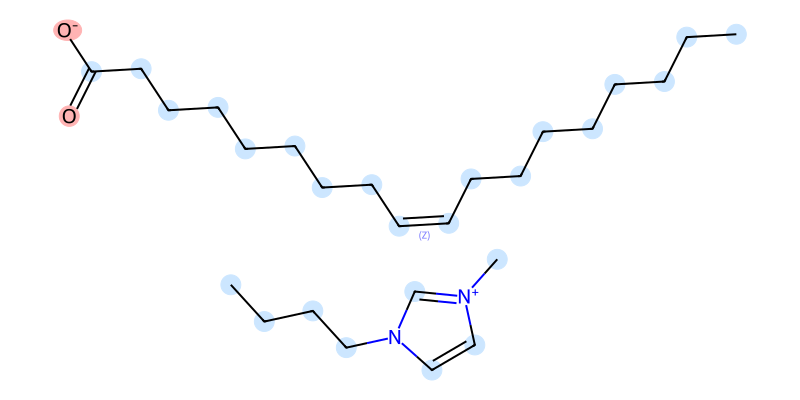
\includegraphics[width=0.55\textwidth]{figures/fig_bmim_oleate.png}
\caption{[BMIM][oleate], one of the two bio-based candidate ILs considered in this work.}
\label{fig:oleate}
\end{figure}
